% This is "sig-alternate.tex" V2.0 May 2012
% This file should be compiled with V2.5 of "sig-alternate.cls" May 2012
%
% This example file demonstrates the use of the 'sig-alternate.cls'
% V2.5 LaTeX2e document class file. It is for those submitting
% articles to ACM Conference Proceedings WHO DO NOT WISH TO
% STRICTLY ADHERE TO THE SIGS (PUBS-BOARD-ENDORSED) STYLE.
% The 'sig-alternate.cls' file will produce a similar-looking,
% albeit, 'tighter' paper resulting in, invariably, fewer pages.
%
% ----------------------------------------------------------------------------------------------------------------
% This .tex file (and associated .cls V2.5) produces:
%       1) The Permission Statement
%       2) The Conference (location) Info information
%       3) The Copyright Line with ACM data-intensive
%       4) NO page numbers
%
% as against the acm_proc_article-sp.cls file which
% DOES NOT produce 1) thru' 3) above.
%
% Using 'sig-alternate.cls' you have control, however, from within
% the source .tex file, over both the CopyrightYear
% (defaulted to 200X) and the ACM Copyright Data
% (defaulted to X-XXXXX-XX-X/XX/XX).
% e.g.
% \CopyrightYear{2007} will cause 2007 to appear in the copyright line.
% \crdata{0-12345-67-8/90/12} will cause 0-12345-67-8/90/12 to appear in the copyright line.
%
% ---------------------------------------------------------------------------------------------------------------
% This .tex source is an example which *does* use
% the .bib file (from which the .bbl file % is produced).
% REMEMBER HOWEVER: After having produced the .bbl file,
% and prior to final submission, you *NEED* to 'insert'
% your .bbl file into your source .tex file so as to provide
% ONE 'self-contained' source file.
%
% ================= IF YOU HAVE QUESTIONS =======================
% Questions regarding the SIGS styles, SIGS policies and
% procedures, Conferences etc. should be sent to
% Adrienne Griscti (griscti@acm.org)
%
% Technical questions _only_ to
% Gerald Murray (murray@hq.acm.org)
% ===============================================================
%
% For tracking purposes - this is V2.0 - May 2012

%\documentclass{acm_proc_article-sp}
\documentclass{sig-alternate}
\usepackage{color}
\usepackage{multirow}
\usepackage{listings}
\usepackage{url}
\usepackage{dblfloatfix}
\usepackage{fixltx2e}
\usepackage{balance}
\usepackage{listings}
\lstset{language=sql, escapeinside={\$}, basicstyle=\small, mathescape, escapeinside={\%*}{*)}}

\newtheorem{theorem}{Theorem}[section]
\newtheorem{corollary}{Corollary}[theorem]

\newif\ifdraft
\drafttrue
%\draftfalse                                                                              
\ifdraft
\newcommand{\zhaonote}[1]{{\textcolor{cyan}    { ***Zhao:      #1 }}}
\newcommand{\evannote}[1]{{\textcolor{red}    { ***Evan:      #1 }}}
\newcommand{\note}[1]{ {\textcolor{red}    {\bf #1 }}}
\else
\newcommand{\zhaonote}[1]{}
\newcommand{\evannote}[1]{}
\newcommand{\note}[1]{}
\fi

\newenvironment{shortlist}{
        \vspace*{-0.5em}
  \begin{itemize}
  \setlength{\itemsep}{-0.1em}
}{
  \end{itemize}
        \vspace*{-0.5em}
}
\newcommand{\up}{\vspace*{-1em}}

\begin{document}

\title{Diagnosing Machine Learning Pipelines with Fine-grained Lineage}

%\numberofauthors{1} 
%\author{
%\alignauthor Zhao~Zhang, Evan~R.~Sparks, Michael~J.~Franklin \\\
%       \affaddr{AMPLab, University of California, Berkeley}\\
%       \email{\{zhaozhang, sparks, franklin\}@cs.berkeley.edu} 
%}

\maketitle

\begin{abstract}
We present the SystemX lineage system to enable the diagnosis of distributed machine learning (ML) pipelines by leveraging the fine-grained
data lineage.  
SystemX exposes a concise yet powerful API, derived from \emph{primitive lineage types}. 
It captures fine-grained data lineage for each  data transformation by recording the input datasets, the output datasets and the cell-level mapping between them. 
It also collects all information that is needed to reproduce the computation.
SystemX efficiently enables data anomaly removal and computation replay, code debugging, and result analysis.
For a single transformation, SystemX's high-order function approach can reduce the storage consumption by up to 
45x compared to the baseline of element-wise mapping recording.
Using the spatial index allows SystemX to speed up lineage query performance by a further 2x-31x. 
SystemX can answer the real use case lineage queries within a few seconds, 
which is low enough to enable interactive diagnosis of ML pipelines.
\end{abstract}

% A category with the (minimum) three required fields
\category{Data management systems}{Database design and models}{Data model extensions}[Data provenance]
%\keywords{ACM proceedings, \LaTeX, text tagging}

\section{Introduction}
Machine learning frameworks are increasingly popular as practitioners and researchers can quickly
build applications (referred to as ML pipelines or pipelines in the rest of this paper) with a high-level 
programming language to pipeline data preparation, feature extraction, model training, and prediction. 
Among these systems, Scikit-learn~\cite{pedregosa2011scikit}
is a single-computer-based framework while TensorFlow~\cite{tensorflow15}, Apache Mahout~\cite{owen2011mahout}, MLlib~\cite{meng2015mllib}, 
SystemML~\cite{ghoting11systemml}, and KeystoneML~\cite{sparks15} focus on a distributed environment.

In practice, to obtain a working model, users often need to try a number of options (e.g., featurization, training parameters, and datasets). 
When experimenting with these options, users frequently analyze results together with the corresponding input data,  
locate code segment responsible for unexpected outcomes, or rerun the computation with the removal of suspicious data anomalies.
Commonly they use a case-by-case solution to record necessary information and store such information in persistent storage for examination.
These solutions are often use case specific, prone to performance degradation, and they can complicate code
management due to the demand for multiple versions of a pipeline.
Given that this is a commonly repeated work pattern, it is natural to add support for ML pipeline diagnosis.

In this paper, we describe the design of a diagnostic system for distributed ML frameworks by leveraging fine-grained data lineage.
Compared to coarse-grained lineage at file or relational table metadata level, fine-grained lineage is at the data structure cell level, e.g., elements in a matrix. 
We assume an ML framework with a programming model that abstracts a pipeline as a chain of data transformations, such as KeystoneML
which builds on top of Apache Spark~\cite{zaharia12}, and use two building blocks: {\bf transformers} and {\bf estimators}.
A {\bf transformer} applies a deterministic unary function to data items and produce new ones.
An {\bf estimator} takes a collection of data items, feeds them to a training procedure,  and produces a {\bf transformer}.
We choose this model because it allows users to declare and instrument lineage capturing directly in the transformer.
Our diagnostic system provides:
\begin{shortlist}
\item{} A flexible interface for users to instrument how and what to capture
\item{} Low overhead for capturing and storing lineage
\item{} Low latency for lineage queries to enable interactive pipeline diagnosis
\end{shortlist}
%This diagnostic system enables users to specify the data transformation lineage with a concise interface, customize the instrumentation, 
%capture fine-grained lineage with a minimal performance penalty, and serve the lineage query 
%(e.g., query the input elements that contribute to an output element) with a low latency. 

%answer sophisticated lineage query responsively( with query latency lower than 10~seconds~\cite{nielsen2009}).
Lineage tracking has been investigated in many contexts.
Existing systems such as Chimera~\cite{foster02} and Taverna~\cite{oinn02} can collect coarse-grained lineage 
at the level of files and computations for scientific workflow systems.
The weak inversion and verification methods~\cite{woodruff97} for the RDBMS-based visualization systems 
were proposed to track approximate lineage.
%DeepDive~\cite{shin15} explores approximate inference for the incremental maintenance problem in the context of knowledge base system.
Data warehouse fine-grained lineage capturing and serving is enabled by the works of Cui and Widom~\cite{cui00, cui03}.
Trio~\cite{widom04} records lineage for the RDBMS at query execution time.
RAMP~\cite{ikeda11, park11} and Newt~\cite{logothetis13} present
solutions for MapReduce systems, and capture lineage on low level operators such as mappers and reducers.
SubZero~\cite{wu13}, which is built on SciDB~\cite{brown10}, has a similar lineage capturing interface on predefined operators and UDFs.

Unfortunately, these existing lineage tracking systems are not suitable for the distributed ML frameworks for three reasons.
First, the coarse-grained lineage information collected by scientific workflow systems (e.g., Chimera) lacks the necessary detail of cell-level mapping.
Second, approximate approaches, such as the weak inversion and verification methods, 
relax lineage accuracy thus cannot be used for diagnosing the correctness of ML pipelines.
Third, the lineage capturing interface of Trio, RAMP, Newt, and SubZero is designed for
the underlying system operators (e.g., SQL operators for RDBMS, aggregate-select-project-join operators in data warehouse, 
mappers and reducers in MapReduce systems, and pre-defined operators and UDFs in SciDB). 
In contrast, ML frameworks do not have such a set of well-defined low level operators,
which makes it difficult to design a general lineage capturing interface.
%This approach is general for all workloads running on the system and completely transparent to users, 
%thus it gives users very limited flexibility for customized instrumentation (specification of lineage type and the data to be collected) 
%in the case even if users know the exact data to collect.
Other challenges of building an ML framework diagnostic system include the cost introduced by 
lineage capturing and the low latency requirement for lineage queries to enable interactive diagnosis.
Table~\ref{tb:overhead} shows the performance penalty incurred by lineage in recent work.

\begin{table}[t]
\begin{center}
    \caption{Performance Penalty Reported by Existing Lineage Systems}
    \begin{scriptsize}
    \begin{tabular}{ | c | c | c |}
    \hline
    Project & Underlying System & Perf Penalty  \\ \hline \hline
    RAMP~\cite{ikeda11} & Hadoop~\cite{HADOOP} & 16-76\% \\ \hline
    Newt~\cite{logothetis13} & Hadoop~\cite{HADOOP} & 20-50\% \\ \hline
    SubZero~\cite{wu13} & SciDB~\cite{brown10} & 50\%-150\% \\ \hline
    %SystemX & KeystoneML~\cite{sparks15}, Spark~\cite{zaharia12} & 16\%-54\% \\ \hline
    \end{tabular}
    \end{scriptsize}
    \label{tb:overhead}
\end{center}   
\end{table}

Because ML pipeline builders have deep understanding of data transformations,  
we present a lineage capturing interface that lets users decide what data to capture and how to capture it.  
By formulating the cell level mapping of an ML pipeline as a sequence of multi-dimensional space transformations
(Figure~\ref{fig:conceptual} shows a conceptual illustration), we identify seven primitive lineage types.
Higher-dimensional spaces can collapse/flatten to lower-dimensional spaces along one dimension at a time, 
resulting in {\bf collapse} mapping (\textcircled{1}) and {\bf flatten} mapping (\textcircled{6}, \textcircled{7}). 
A mapping between spaces with the same number of dimensions can be {\bf identity} mapping (\textcircled{5}), {\bf all} mapping (\textcircled{9}), 
{\bf geometry} mapping (\textcircled{2}, \textcircled{4}), {\bf lincom} (short for linear combination) mapping (\textcircled{3}, \textcircled{8}),
or {\bf join} mapping. 
These seven mapping types cover 87\% (39 out of 45) of the data transformations in the current code base of KeystoneML~\cite{sparks15}. 
For transformations that are not covered, the lineage capturing interface allows users to specify customized mapping functions.
A formal definition of the mapping types is in \S\ref{sec:Map-Func}.

\begin{figure}[t]
\begin{center}
    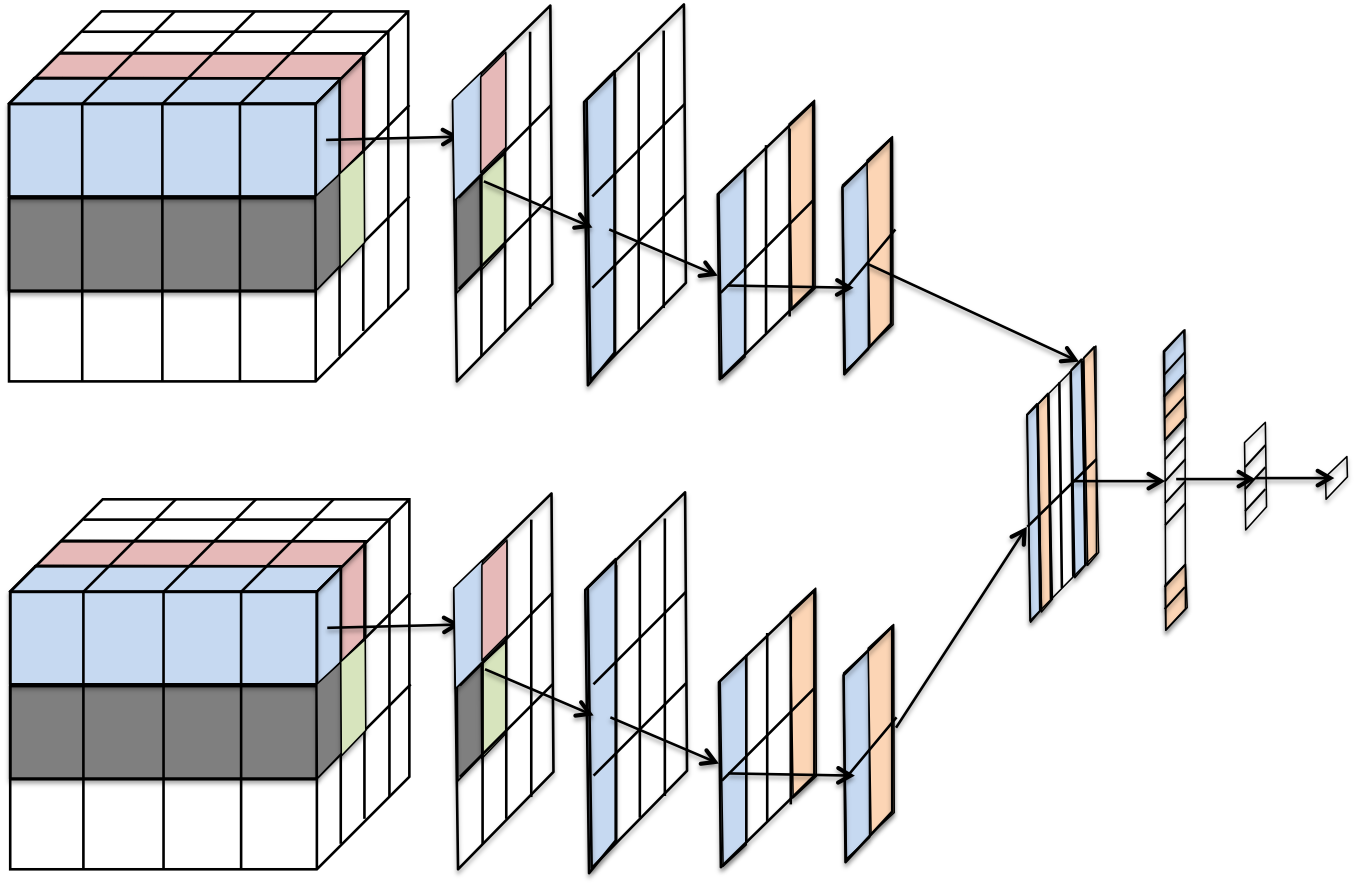
\includegraphics[width=85mm]{pictures/Conceptual}
    \caption {A synthetic image classification pipeline with elements mapping highlighted in color scheme. 
    \textcircled{1}: Conversion of multi-channel image to gray scale.
    \textcircled{2}: Local feature extraction.
    \textcircled{3}: Vector dimension reduction.
    \textcircled{4}: Vector sampling.
    \textcircled{5}: Conversion from float to double.
    \textcircled{6}: Vector combining.
    \textcircled{7}: Matrix vectorizing.
    \textcircled{8}: Linear model prediction.
    \textcircled{9}: Selection of the index with maximum value.
    \label{fig:conceptual}
}
\end{center}
\end{figure}


In this paper, we present SystemX\footnote{This name is a place holder for double-blind review}, a lineage capturing and serving system that implements the above general solution.
SystemX is integrated with the open source KeystoneML distributed machine learning framework.
SystemX interacts with KeystoneML at the transformer level, where users can declare the lineage type and customize instrumentation.
SystemX exploits the  data structure metadata (e.g., the size of each dimension of a space) when recording mappings to reduce storage overhead.
It also uses a high-order function approach and spatial index for geometry mappings that do not have a regular mapping pattern.
SystemX collects six types of data for each transformer: the input dataset, the output dataset, the mapping between them
along with the computation, the optional model and random factor.
SystemX stores the lineage information on HDFS~\cite{shvachko10} via the resilient distributed dataset (RDD) abstraction
of Apache Spark~\cite{zaharia12} (the underlying computing engine of KeystoneML).
Unlike Spark lineage, which tracks partition-level data dependency and associated computation for internal system resilience,
SystemX tracks lineage with a finer granularity at the cell level of data structures.
In addition, SystemX exposes an interface for users to specify lineage types and to query the lineage.
When queried, SystemX can load the lineage information from storage and reconstruct the lineage chain.
Users have the flexibility to reconstruct a single transformer lineage, a partial or whole chain.

SystemX enables lineage-based ML pipeline diagnostics such as code validation, results inspection, and data cleaning.
A detailed discussion of these three use cases is presented in \S\ref{sec:Back-cases}.
Compared to the naive solution of materializing cell-wise mapping, 
SystemX's techniques (spatial index and high-order function) enable 2x-31x speedups at lineage query time.
This new capability comes at the cost of performance overhead during pipeline training/execution.
The overhead is measured in wall clock time, memory consumption, and storage space.
For the three use cases, the wall clock time overhead for lineage capturing is 16\%-54\%, which is comparable to other distributed lineage systems
summarized in Table~\ref{tb:overhead}.
SystemX increases memory usage by 31\%-79\%,
and the storage space for lineage information varies case by case from $\sim$100~MB to $\sim$1~TB.


In summary, we make the following contributions:
\begin{shortlist}
\item{} We design a concise and powerful lineage system interface by formulating the cell-wise mapping in ML pipelines as multi-dimensional space transformations.
\item{} We introduce a high-order function approach for describing the geometry to reduce storage overhead.
\item{} We present a spatial index solution to speed up geometry mapping queries and evaluate a set of spatial indexing strategies.
\item{} We present and analyze three real use cases of using fine-grained data lineage for code validation, results inspection, and data cleaning, respectively.
\end{shortlist}

\section{S\MakeLowercase{ystem}X Framework}
\label{sec:functional}
Two basic functions of SystemX are lineage capturing and serving.
SystemX requires a programming interface between users and the lineage capturing unit. 
This interface should be concise with a few variations and options.
This interface should also be powerful in terms of data transformation coverage.
This interface should be flexible so that users can decide how the lineage should be captured and what datasets to be captured.

The serving unit requires a user interface for lineage query.
Users should be able to construct the pipeline lineage by chaining that of each transformer.
SystemX should provide the forward query ({\bf qForward()}) and backward query ({\bf qBackward()}) functionality.
%The single transformer lineage should be able to be replayed deterministically, meaning that with the same input dataset and transformer,
%the lineage contains enough information with which users can reproduce the results.

Lineage capturing in SystemX should add a minimal wall clock time overhead, memory usage and storage space.
To enable interactive diagnosis, SystemX should be able to answer lineage queries with low latency.
According to the report~\cite{nielsen2009}, 
1~second in a human computer interaction system is considered to be the boundary of keeping a user's thought flow while 
10~seconds is considered as the boundary to lose a user's attention.

\subsection{Pipeline and Datasets}
\label{sec:Map-Pipe-Data}
A dataset $I$ is defined as a collection of structured data. In the scope of this work, the supported structures are: 
string, vector, matrix, and image, while users can define data structures with higher dimensions.
A vector or a string is a one dimensional data structure and a matrix is two dimensional. 
For simplicity, a string is viewed as a vector.
An image is a three dimensional data structure that is defined by the height, the width and the number
of channels. 

An element $e \in I$ has two properties: coordinate $e.Coor$ and value $e.Value$. 
Combining the additional dimension in the collection (RDD or sequence) with the data structure, 
the coordinate of an element can be a pair, a triple, or a quadruple of integers
for vector, matrix, and image, respectively.

A pipeline $P$ is defined as a sequence of transformers $(T_1, T_2, ..., T_n)$. 
Each transformer $T_i$ takes a dataset $I_i$ as its input, and produces $I_{i+1}$ as the output: 
$I_{i+1} = T_i(I_i)$. 
Especially, the output of the whole pipeline is denoted as $O = I_{n+1}$

To simplify the discussion, we use a vector collection (a 2D space) as the input and output data structures as the example.
Also we only present the definition of forward query given that 
backward query can be derived by reversing the table order in the join operation.

\subsection{Dataset and Mapping}
\label{sec:formal-ds-mapping}
Conceptually, the input dataset and output dataset can be defined
as tables with each element's coordinate in the data structure as key.
\begin{lstlisting}
input(Coor:(Int,Int), Value:Double)
output(Coor:(Int,Int), Value:Double)
\end{lstlisting}

The mapping between the input and output dataset is a left outer join of the two tables with a mapping function.
The Func() function returns the corresponding output elements given an input element. 
It is a left outer join since an input element may not be corresponding to any output element.
\begin{lstlisting}
SELECT * FROM input
LEFT OUTER JOIN output 
    ON Func(input.Coor) $\ni$ output.Coor;
\end{lstlisting}

In practice, SystemX separates the metadata from the actual element values and record metadata mapping
in a table.
\begin{lstlisting}
mapping(inCoor:(Int,Int), outCoor:(Int,Int))
\end{lstlisting}

\begin{lstlisting}
INSERT INTO mapping
SELECT input.Coor, output.Coor FROM input
LEFT OUTER JOIN output 
    ON Func(input.Coor) $\ni$ output.Coor;
\end{lstlisting}

The retrieval of actual element values can be obtained by joining the mapping table and the output dataset table.
\begin{lstlisting}
SELECT mapping.outCoor, output.Value
FROM mapping
LEFT OUTER JOIN output 
    ON mapping.outCoor = output.Coor;
\end{lstlisting}

The input and output mapping of a pipeline is in turn a sequence of mappings of individual transformer.
Consider a pipeline $P=(T_1, T_2, ..., T_n)$, we denote $mapping_i$ as the mapping table for transformer $T_i$.
The mapping of the pipeline is a sequence of left outer join operations of $\{mapping_1, ..., mapping_n\}$ 
on $mapping_i.outCoor = $\\$mapping_{i+1}.inCoor$.

\subsection{Mapping Function}
\label{sec:Map-Func}
The mapping function {\bf Func()} contains the core information of the input and output element dependency.
Recording the element-wise dependency can take up to $O(kN^2)$ space given k N-element vectors in the case
of every output element depending on every input element. 
To eliminate this polynomial explosion in space requirements, we identify seven primitive mapping functions.
From higher dimension space to lower dimension space, the mapping can be {\bf collapse} or {\bf flatten}.
Between the equal dimension spaces, the mapping can be {\bf identity}, {\bf all}, {\bf geometry}, {\bf lincom}, and {\bf join}.
Figure~\ref{fig:narrowmapping} shows the seven primitive mapping functions, with the mapping highlighted with color scheme.

\begin{figure}[t]
\begin{center}
    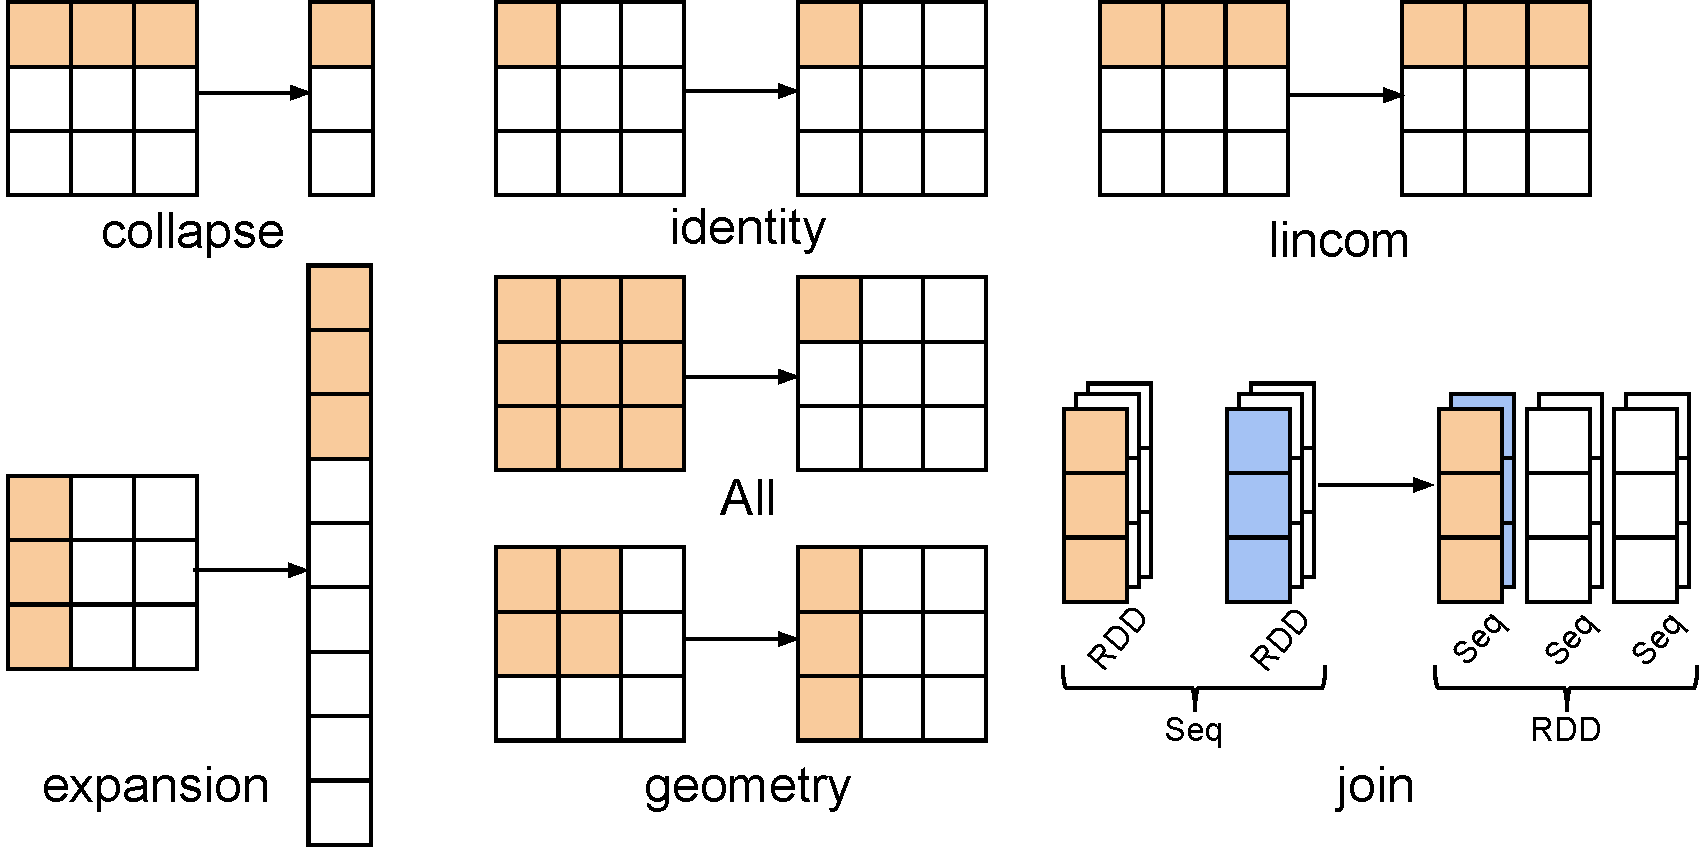
\includegraphics[width=85mm]{pictures/narrowmapping}
\caption {Seven primitive mapping functions.
    \label{fig:narrowmapping}
}
\end{center}
\end{figure}

{\bf Collapse} mapping describes a space collapsing into a lower space along one dimension which needs
to be specified by the user. Examples include gray scaling a multiple channel image.
{\bf Flatten} mapping is where a space flattens to a one-dimension lower space, e.g., flattening a matrix to a vector with column major.
In {\bf identity} mapping, each output element only depends on the element with the identical coordinate in the input matrix.
In {\bf all} mapping, each output element depends on all elements in the input matrix.
{\bf Geometry} mapping describes the case where a group of output elements depend on a group of input elements.
{\bf Lincom} mapping describes the data dependencies in a linear model.
{\bf Join} mapping happens between equal dimension space transformation. The example in Figure~\ref{fig:narrowmapping} 
is a transformation from a sequence of a vector collection (RDD) to a collection (RDD) of vector sequence by joining the vectors
on the collection (RDD) position.
For the mappings that are not covered by the primitive functions, SystemX allows users to define their own mapping functions.

\subsection{Mapping Query}
A forward query with a key  ({\bf qForward(key)}) over the mapping of a transformer or a pipeline can be expressed as:
\begin{lstlisting}
SELECT outCoor FROM mapping
WHERE key = inCoor;
\end{lstlisting}

A forward query with a list of $keys=\{k_1, k_2, ..., k_n\}$ ({\bf qForward(keys)}) can be expressed as:
\begin{lstlisting}
SELECT outCoor FROM mapping
WHERE $k_1$ = inCoor OR ... OR $k_n$ = inCoor;
\end{lstlisting}

\section{K\MakeLowercase{eystone}ML and Use Cases}
\label{sec:Background}
A brief review of KeystoneML is presented to help understand the technical background of this work.
To motivate SystemX, we present three representative use cases of using fine-grained lineage for ML pipeline diagnostics.

\subsection{KeystoneML}
In principle, SystemX is general for distributed ML frameworks whose programming interface can be abstracted as transformers and estimators.
We integrate SystemX with KeystoneML to show the effectiveness of the design.
KeystoneML is an application framework designed for the implementation of robust large-scale machine learning pipelines. Built on the principles of declarative programming and modular design, KeystoneML provides a light-weight and elegant API that allows users to describe these pipelines as the composition of two types of operator--transformers, which perform deterministic data transformation, and estimators, which ``learn'' transformers based on training data. KeystoneML pipelines are fit and executed in parallel using Apache Spark. These pipelines are compiled into an application directed acyclic graph (DAG) and optimized before execution. Current optimizations include online decisions about intermediate state materialization, as well as standard optimizations such as common subexpression elimination. KeystoneML includes a library of standard feature extractors in domains including computer vision, audio, and text processing, as well as standard statistical procedures and Estimators for several types of machine learning model.

\subsection{Use Cases}
\label{sec:Back-cases}
The three use cases come from real ML pipelines of image classification and astronomy image processing. 
These three cases are representative of code validation, results inspection, and data cleaning, respectively.

\subsubsection{Code Validation}
In this case we use lineage for the debugging process as pipelines change and are augmented. 
Typical machine learning workflows are constructed via an iterative process of refinement with a machine learning developer or data scientist in the loop.
These users are constantly engineering new features, adding new datasources, and trying out new machine learning methods at all stages of the pipeline.
Lineage offers a natural way for these users to hone in on the areas where two similar pipelines diverge in terms of their intermediate data, and presents a new avenue for investigation of model performance by allowing users to pinpoint the point at which their data diverged from a known good pipeline and to inspect \emph{what} changed during the data processing procedure. 


\begin{figure*}[t]
\begin{center}
    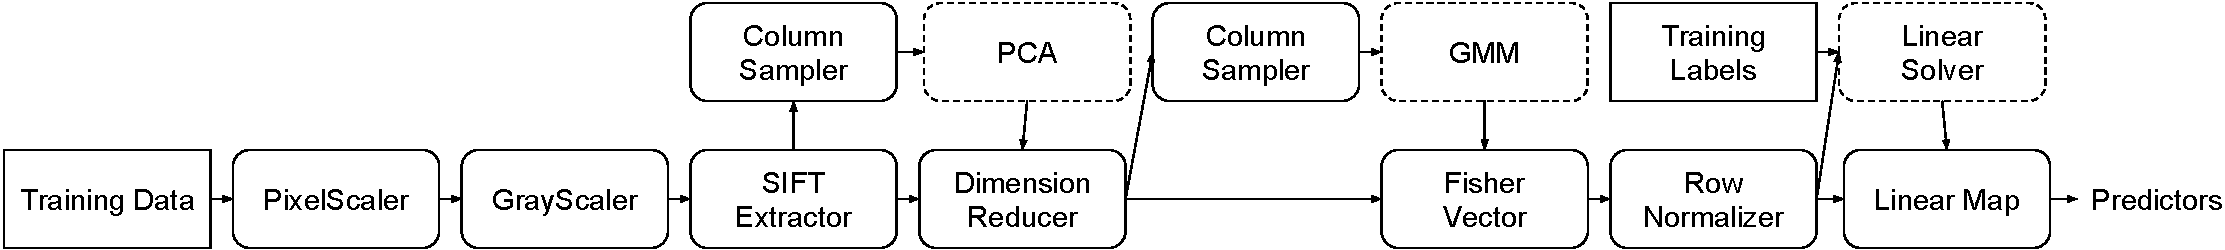
\includegraphics[width=150mm]{pictures/VOCSIFTFisher}
    \caption {The SIFTFisher pipeline, boxes are dataset, rounded-corner boxes are transformers, dashed rounded-corner boxes are estimators.
    \label{fig:vocsiftfisher}
}
\end{center}
\end{figure*}

As a concrete example, consider the SIFTFisher pipeline, shown as Figure~\ref{fig:vocsiftfisher}. 
It has been shown that augmenting traditional SIFT~\cite{lowe99} (Scale-invariant feature transform) descriptors 
with their locations in the input image can improve classification performance.
However, when we first developed such a pipeline, our results conflicted with published work indicating that these features provided a statistically significant improvement in classification accuracy.
By employing lineage based debugging, we could isolate exactly where in the pipeline our calculations diverged from the original features, and diagnose impacts seen downstream like an under-fit GMM (Gaussian Mixture Model), and trace the ultimate lack of classification improvement to a bug in the underlying C library which we called into.
By visualizing the features we could see that the new features added to our model did not correspond to positions in the image, but rather contained values outside of a suitable range for these features, which turned out to be randomly allocated memory. 
The SIFT feature visualization involves a  backward query on the SIFTExtractor transformer lineage. 

\begin{lstlisting}
mapping(inCoor:(Int,Int,Int),outCoor:(Int,Int,Int))

SELECT inCoor FROM mapping WHERE outCoor = key;
\end{lstlisting}

\subsubsection{Results Inspection}
Fine-grained data lineage of ML pipelines enables results interpretation, potential data anomaly detection, 
and retrospection of supporting input data.

\begin{figure}[ht]
\begin{center}
    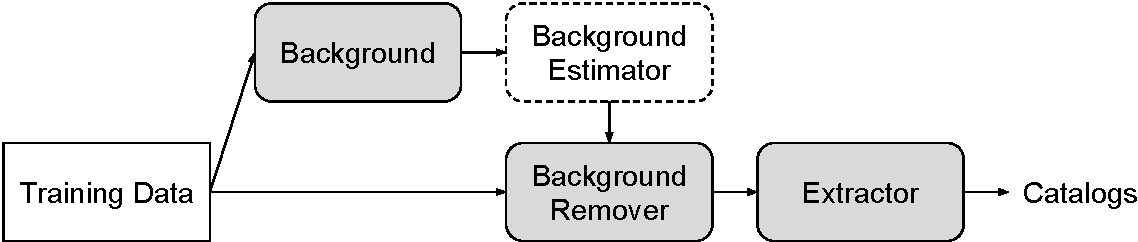
\includegraphics[width=85mm]{pictures/SourceExtractor}
    \caption {The SourceExtractor pipeline, boxes are dataset, rounded-corner boxes are transformers, dashed rounded-corner boxes are estimators.
    \label{fig:sourceextractor}
}
\end{center}
\end{figure}

One such use case is results inspection in the SourceExtractor pipeline, shown in Figure~\ref{fig:sourceextractor},
that processes telescope images and produces astronomical object catalogs. 
The astronomical object catalog includes the position, shape, and other statistical properties of the object.
In this case, astronomers find the bright objects over a threshold and validate that these objects are indeed astronomical objects rather
than noise caused by cosmic rays.
With the lineage information, astronomers can first filter the results to find the objects whose brightness is above a threshold.
Then using backward query, they can find corresponding pixels for these bright objects. 
Either through mathematical analysis or human intervention, they are able to validate the correctness of the bright objects.
Then the astronomer can use forward query to figure out how a bad pixel propagates to the atalogs.
The backward query for this use case can be expressed as following.
\begin{lstlisting}
output(Coor:(Int,Int,Int),Brightness:Double)
mapping(inCoor:(Int,Int,Int),outCoor:(Int,Int,Int))

SELECT mapping.inCoor FROM mapping 
LEFT OUTER JOIN output
  ON mapping.outCoor = output.Coor
WHERE output.Brightness > threshold;
\end{lstlisting}

The forward query on the bad pixel propagation can be translated into the following code.
\begin{lstlisting}
SELECT outCoor FROM mapping WHERE inCoor = key;
\end{lstlisting}

\subsubsection{Data Cleaning}
\label{sec:Back-Case-Cleaning}
Another use of the lineage information is for users to apply a subset of the prepared dataset to fit the model. 
The ML expert who is building a SIFTFisher pipeline, shown in Figure~\ref{fig:vocsiftfisher}, identifies bad 
training data items (e.g., the images that have both dogs and cats) due to measurement error. 
A natural investigation is then to remove these images, and test if that improves prediction accuracy.

With SystemX, the user can intercept the pipeline by loading the output of RowNormalizer (the last transformer before training process) 
directly into KeystoneML, filter out the data items that are derived from the images with both dogs and cats , 
and apply the filtered dataset directly to the linear solver.
In this way, the rerunning process can bypass the expensive data preparation procedure (from PixelScaler to RowNormalizer) 
resulting in shorter turnaround time.
Without lineage information, the user has to remove the according images from the training set and rerun data
preparation part (from PixelScaler to RowNormalizer), then feed the dataset to linear solver to train the model.



%\section{Formal Discussion}
%\label{sec:Mapping}
%In this section, we formally define the notion of an ML pipeline, dataset, mapping and its associated operations of query in the context of 
%relational database.


%\subsection{Data Preparation Skipping}
%\label{sec:formal-skipping}
%In use cases such as data cleaning presented in \S\ref{sec:Back-Case-Cleaning}, users want
%to remove certain suspicious input data items that might relate to bad prediction results and retrain the model then
%test its performance. 
%Repeating the data preparation steps (e.g., from PixelScaler to RowNormalizer in SIFTFisher pipeline) incurs
%long running time.
%One natural thought in such case is ``can we skip the computation applied on the unchanged data items by removing
%the corresponding prepared data items directly?''
%
%Formally, given a data transformation {\it f()} applied on a set $C$ of vectors \{$v_1, v_2, ..., v_n$\}.
%we say it is safe to remove {\it f($v_i$)} if {\it $f(C \setminus {v_i})) = f(C) \setminus {f(v_i)}$}.
%In other words, function {\it f()} is distributive on vectors \{$v_1, v_2, ..., v_n$\}. 
%With single or few transformers, users are able to track the distributive property.
%However when the pipeline is deep, such a property is hard to track.
%
%Using the fine-grained data lineage, we present a validation method for the distributive property.
%The mapping of {\it f()} is self-contained if $qBackward_f(qForward_f(v_i)) \subseteq v_i$, where vector $v_i$ can be viewed 
%as a set of one-dimensional elements.


%\begin{theorem}
%\label{thm:distributive}
%A data transformation f() is distributive if the mapping of f() is self-contained.
%\end{theorem}

%\begin{proof}
%By contradiction, assume f() is not distributive on collection $C$ of vectors  \{$v_1, v_2, ..., v_n$\}, then $\exists e \in v_j $ s.t. $f(v_i)$ takes as input.
%Then $e \in qBackward_f(qForward_f(v_i))$ and $e \in v_i$ which results in  $qBackward_f(qForward_f(v_i)) \nsubseteq v_i$, which contradicts the assumption.
%\end{proof}

%\begin{corollary}
%A sequence of data transformations ($s = {f_1, f_2, ..., f_n}$) is distributive if the mapping between the very input and output datasets is self-contained.
%\end{corollary}


%Since transformers operate at the data structure (vector, matrix, image) level, we use the notation
%$\overline{I_i(e)}$ as the companion of $I_i$ with respect to element $e$ such that $\forall a \in \overline{I_i(e)}$,
%\[ a.value =
%  \begin{cases}
%    e.value       & \quad \text{if } a.coor = e.coor\\
%    NaN  & \quad \text{otherwise}. \\
%  \end{cases}
%\]

%Accordingly, given a list of distinct elements $(e_1, ..., e_m)$, the companion of $I_i$ with respect to $(e_1, ..., e_m)$ is
%described as: $\forall a \in \overline{I_i(e_1, ..., e_m)}$, 
%\[ a.value =
%  \begin{cases}
%    e.value       & \quad \text{if } \exists e \in (e_1,...,e_m), a.coor = e.coor\\
%    NaN  & \quad \text{otherwise}. \\
%  \end{cases}
%\]

%Before defining the lineage, we need to introduce the relationship between the two data structures $A$ and $B$ with the same type.
%We say $A \subseteq B \text{ or } B \supseteq A$, $\text{if }\forall a \in A, \exists b \in B, s.t.\text{ } a \neq NaN \land a.coor = b.coor \land a.value = b.value$.
%By saying $A = B$, we mean $A \subseteq B$ and $B \subseteq A$.
%
%We define the data lineage of a given element as the elements in the input dataset that is used to produce present element.
%The single transformer lineage is
%\begin{equation}
%S(e \in I_{i+1}) = \{e_1, ..., e_m | T_i(\overline{I_i(e_1, ..., e_m)}) \supseteq \overline{I_{i+1}(e)}\}.
%\label{equa:SingleLineage}
%\end{equation}
%
%Recursively, the lineage of a given element across multiple transformers can be defined as
%\begin{equation}
%L(e) = \cup_{e' \in S(e)} L(e').
%\end{equation}
%
%We define the property 
%\begin{equation}
%Replay(e \in I_{i+1}) = \overline{I_{i+1}(e)} \subseteq T_i(\overline{I_i(e_1, ..., e_m)})
%\end{equation}
%as the replay property, which means we can reproduce an output element $e$ by applying the corresponding transformer to its data lineage.
%The constraint of the replay property is that only the element $e$ is guaranteed to be the same as the original transformation,
%if $\overline{I_{i+1}(e)} \subset T_i(\overline{I_i(e_1, ..., e_m)})$. 
%In this case, the results of the replayed transformer may produce inconsistent results for elements other than $e$ in $I_{i+1}$. 
%Similarly, the replay property for multiple elements only guarantees the correctness of these elements themselves.
%
%\subsection{Data Lineage Query}
%The forward query of an element over data lineage of a pipeline $P$ returns $qForward(e) = \{e' | e \in L(e' \in O)\}$. 
%And the backward query of an element over data lineage returns $qBackward(e) = e' \in L(e)$.
%Specifically, the identifier of an element is its coordinates in the according data structure, so the query actually takes
%the coordinates of the input element as key, and query over the data lineage. The query that spans multiple transformers 
%use coordinates as intermediate data. Once the query reaches the final transformer, it can associate the actual values
%with the result element coordinates and return them.
%
%Queries of multiple elements can then be expressed as the union of the query for each element: 
%\begin{equation}
%\begin{split}
%qForward(e_1, ..., e_m) = \cup_{e \in (e_1, ..., e_m)} qForward(e) \\
%qBackward(e_1, ..., e_m) = \cup_{e \in (e_1, ..., e_m)} qBackward(e).
%\end{split}
%\end{equation}

%\section{Design Goals}
%\label{sec:Req}
%This performance penalty problem is exacerbated for SystemX, since KeystoneML's distributed computing engine Apache Spark 
%optimizes for in-memory computing and does not write intermediate data to disks unless it is a shuffle operation. 
%Comparing to systems such as Hadoop, the same amount of I/O of SystemX will introduce a more significant penalty.
%By exploiting the advanced techniques for space reduction, we expect SystemX's performance penalty to be comparable to the existing systems.
%
%Lineage information can be massive depending on the pipeline, since the input or the intermediate dataset of a pipeline can be large.
%In some transformers, the mapping between the input elements and output elements does not conform a pattern, e.g., Geometry mapping.
%We need advanced techniques (e.g., a compact description of a set of elements) to reduce the storage explosion introduced by such mappings. 
%
%Using SystemX for ML pipeline diagnosing requires a low-latency interaction between users and the lineage serving unit.
%As documented in the report~\cite{nielsen2009} in human computer interaction, 1~second latency is the boundary to keep users' thought flow while 10~seconds
%is the boundary to loose users' attention.
%We expect SystemX's query latency within the 10~seconds boundary to facilitate users diagnosis on ML pipelines.

\section{Design}
\label{sec:Design}
SystemX is designed as an ML pipeline diagnostic tool. 
It has two units: the capturing unit and the serving unit.
The capturing unit requires a user-friendly, flexible, and powerful interface for lineage type declaration and instrumentation.
Performance wise, the lineage capturing unit should add minimal overhead in running time, memory usage and storage space.
The serving unit should be able to answer lineage queries with low latency to enable interactive diagnostics.

In this section and next, we present the design and implementation to address the above goals.

\subsection{Overview}
Figure~\ref{fig:architecture} shows the overview of SystemX and its interactions with other components. 
Rounded-corner rectangles are components around and inside KeystoneML. 
The two-sided arrows indicate interactions between components.
Users compose machine learning pipelines with KeystoneML and submit the compiled DAG to Spark.
All computation and I/O are done through the Spark Resilient Distributed Dataset (RDD) abstraction.
With SystemX, users can declare and instrument lineage at the transformer level, 
so that the compiled DAG also contains lineage capturing and storing operations.
Lineage in SystemX is stored to HDFS~\cite{shvachko10} via Spark's RDD abstraction.
SystemX can load the stored lineage in HDFS to Spark interactive command line interface.
By interacting using the query interface, users can query elements of interest, replay transformation, or analyze
the lineage for other purposes.

\begin{figure}[h]
\begin{center}
    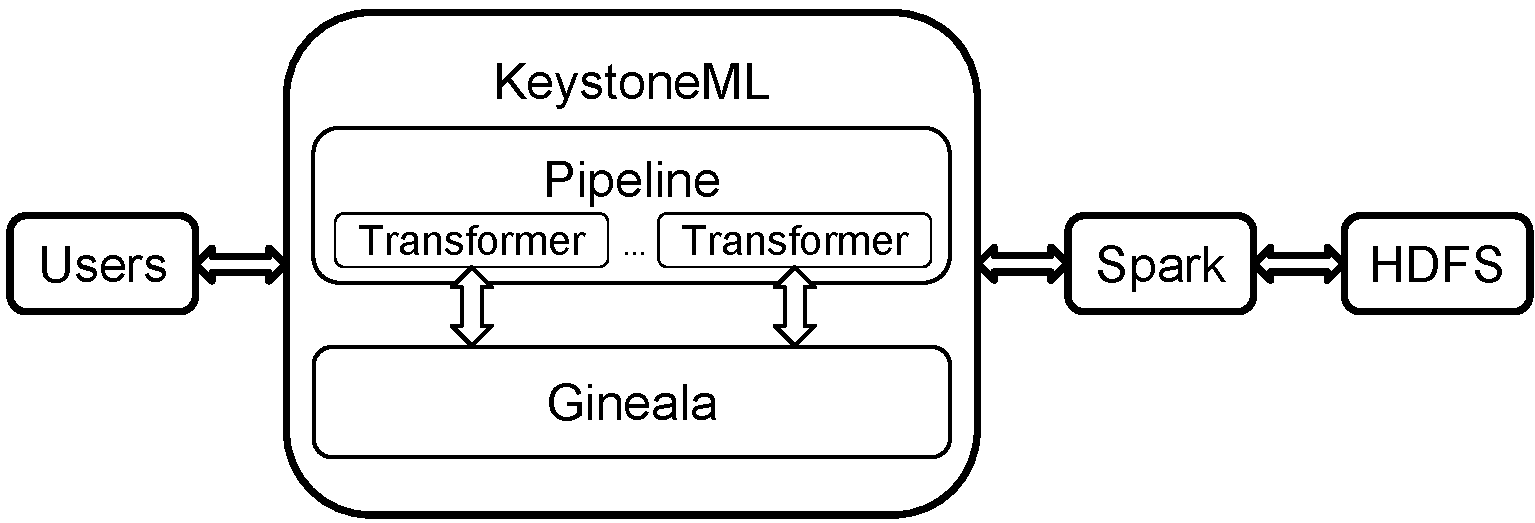
\includegraphics[width=85mm]{pictures/architecture}
\caption {Overview of SystemX and its surrounding components.
    \label{fig:architecture}
}
\end{center}
\end{figure}

\subsection{Lineage Interface}
\label{sec:Design-Lineage}
SystemX exposes the lineage capturing interface by naming the lineage type specific class with its mapping types between input and output datasets.
All the type specific class inherits an abstract class of Lineage, which define common methods shared among the type specific classes:
\begin{shortlist}
\item{} qForward(keys: List[Coor]): List[Coor], given a list of element coordinates returns the forward query results on the metadata mapping of the lineage
\item{} qBackward(keys: List[Coor]): List[Coor], given a list of element coordinates returns the backward query results on the metadata mapping of the lineage
\item{} saveMapping(): saves the collection of metadata mappings of a lineage to disks
\item{} saveInput(): saves the input dataset to disks
\item{} saveOutput(): saves the output dataset to disks.
\end{shortlist}


Table~\ref{tb:lineage-interface} summarizes the lineage types and parameters.
\begin{table}[t]
\begin{center}
    \caption{Primitive Lineage Types}
    \begin{scriptsize}
    \begin{tabular}{ | p{8cm}|}
    \hline
    CollapseLineage(in, out, transformer, dimension) \\ \hline 
    FlattenLineage(in, out, transformer, dimension) \\ \hline
    IdentityLineage(in, out, transformer) \\ \hline
    AllLineage(in, out, transformer) \\ \hline
    GeoLineage(in, out, transformer, mappingCollection) \\ \hline
    LinComLineage(in, out, transformer, model) \\ \hline
    JoinLineage(in, out, transformer, dimension) \\ \hline
    CustomLineage(in, out, transformer, fFunc, bFunc, model, rand) \\ \hline
    \end{tabular}
    \end{scriptsize}
    \label{tb:lineage-interface}
\end{center}   
\end{table}

In general the SystemX lineage capturing interface can collect six types of data: 
the input dataset (in), the output dataset (out), the transformer (transformer), 
the collection of mappings (mappingCollection), the model (model), and the random 
parameter (rand).

By checking the input and output dataset, SystemX is able to figure out the metadata of each data structure 
(e.g., the number and size of dimensions) then use it to specify the mapping type parameters.

\subsection{Mapping}
\label{sec:Design-Mapping}
Mapping on the abstract level provides two interfaces: qForward() and qBackward(). Both interfaces
take a list of element coordinates and return the query results accordingly.
A complete mapping types are presented in Table~\ref{tb:mapping-interface}

For every mapping type presented in ~\S\ref{sec:Map-Func} except the {\bf geometry} mapping, 
SystemX infers metadata of data structures automatically. 
The metadata  of a data structure can be one dimensional (with type of Int), two dimensional (with type of (Int, Int)), and etc.
For example, in an {\bf all} mapping between two matrices of 5 rows and 5 columns,
the mapping is recorded as {\it AllMapping(Meta(5, 5), Meta(5,5))}. 
So upon forward query, the mapping returns the coordinates of all 25 coordinates in the output matrix by only looking into the matrix metadata.
SystemX also uses this data structure metadata to check out-of-bound errors if the given key is outside the space of the data structure.

For {\bf geometry} mapping type, the mapping is arbitrary and cannot benefit from data structure metadata, 
Intuitively, users have to pass in the materialized cell-wise mapping. 
This intuitive solution takes a tremendous amount of space in memory and on disks.


\begin{table}[t]
\begin{center}
    \caption{Primitive Mapping Types}
    \begin{scriptsize}
    \begin{tabular}{ | p{8cm}|}
    \hline
    CollapseMapping(inMeta, outMeta, dimension) \\ \hline 
    FlattenMapping(inMeta, outMeta, dimension) \\ \hline
    IdentityMapping(inMeta, outMeta) \\ \hline
    AllMapping(inMeta, outMeta) \\ \hline
    GeometryMapping(inMeta, outMeta, mappingCollection) \\ \hline
    LinComMapping(inMeta, outMeta, model) \\ \hline
    JoinMapping(inMeta, outMeta, dimension) \\ \hline
    CustomMapping(inMeta, outMeta, fFunc, bFunc, model, rand) \\ \hline
    \end{tabular}
    \end{scriptsize}
    \label{tb:mapping-interface}
\end{center}   
\end{table}

\subsection{Geometry Mapping}
\label{sec:Design-GeometryMapping}
To reduce the size of geometry mapping, SystemX uses a high-order function approach to describe the geometries.
As can be seen in the geometry mapping example in Figure~\ref{fig:narrowmapping}, the backward query of an 
output element should return all the input elements in the corresponding geometry. If the output geometry has 
$N$ elements and the input geometry has $N$ elements, the space complexity of storing such a mapping is $O(N^2)$. 
Inspired by the SIFT and the SourceExtractor implementation, each of them processes an input matrix and produces 
thousands of vectors as outputs. An output vector depends on a group of elements in the matrix, and these elements 
form a two dimensional shape. 
For SIFT, the input elements form a circle with a geographical center and the scale as its radius.
Similarly, the SourceExtractor's input elements form an ellipse. 
SystemX uses a high-order function to describe the geometry such as circle and ellipse. 
Thus the mapping between two geometries is expressed as a tuple of two higher-order functions.
The space complexity goes down to O(1).

Since many softwares such as SIFT and SourceExtractor already return the geographical information with the results.
SystemX exposes a simple interface for two dimensional shapes as special cases.
Users can pass in the geographical information directly to declare rectangle, circle, and ellipse.

Using the high-order function makes query difficult. 
Both the input elements and output elements are encoded with high-order functions, 
and there is a list of such function tuple between two data structures.
A forward query that takes an input element as key thus needs to iterate over all input functions and test if the key is in the function or not.
If the key is in an input function, it then returns the mapping output function, and expands the function to a set of coordinates.
The time complexity of query over geometry mapping is then $O(N)$, assuming there are $N$ tuples in the list.
To speedup the query performance, we implement and compare several indexing strategies, and a detailed discussion is in \S\ref{sec:GeometryIndex}.


\section{Implementation}
\label{sec:Impl}
This section discusses the implementation details for lineage space reduction, mapping function inversions, 
generalization of the primitive mapping types, lineage storage, and the geometry mapping indexing strategies.


\subsection{Metadata Separation}
Capturing lineage and storing it results in longer wall clock time compared to the lineage-free case. 
One way to minimize this capturing time is to store less data.
As discussed in \S\ref{sec:formal-ds-mapping}, SystemX separates the metadata of a data structure 
(e.g., the coordinates of elements in a matrix) from the actual data  and leave the options for users to 
instrument what dataset to collect.

However, under the constraint of complete pipeline lineage integrity, a minimal dataset to be captured
is all the metadata mapping of the transformers given that the intermediate and result 
dataset can always be reproduced with the KeystoneML transformer given the its determinism property. 
A profile on the SIFTFisher and SourceExtractor pipeline shows a space reduction by 
13.7x (from 725.6~GB to 109.9~GB) and 2480.9x (from 507.1G to 204.4M), respectively.

\subsection{Mapping Inversion and Extension}
When formulating the cell level mapping of a transformer as a multi-dimensional space transformation, SystemX defines
the mapping in the direction from input to output and name the according lineage type with its mapping type.
In this paragraph, we explain how to infer backward query (the mapping inverse) of the mapping and how SystemX deals
with mappings that are not directly covered by the primitive types.

All mapping, identity mapping, lincom mapping, and join mapping are symmetric, 
meaning the inverse of these mappings are of the same mapping type.
Collapse mapping and flatten mapping are not symmetric, but the mapping inversion can be inferred
given the data structure metadata (the number and size of dimensions of a space). For example, 
in the collapse case shown early in Figure~\ref{fig:narrowmapping}, a matrix with three rows and three columns
collapses into a vector along the row dimension. Thus a mapping inversion of an element of the vector
is all elements in the corresponding row in the matrix. 
The inversion of flatten mapping can also be inferred with simple calculation.
The inversion of geometry mapping is enabled by switching the order of each geometry tuple.


Among the seven mapping types defined in \S\ref{sec:Design-Lineage}, the collapse mapping and flatten mapping
map spaces that have different dimensions. By definition, they only maps from a higher-dimensional space to a lower-dimensional space.
A transformer that reduces a lower-dimensional space to a higher-dimensional space, e.g., transforming a vector into a matrix, can use
the same flatten mapping type for declaration based on the fact that the reverse mapping of this transformation is a
flatten mapping. SystemX can infer the mapping direction with the metadata of data structures 
(the number of dimensions of a space). 
A similar solution is used for the reverse of collapse mapping.

For sampling transformers, e.g., selecting a subset of a vector collection, SystemX implements it as a geometry mapping.
From the input side, there are a list of geometries (rectangles for vectors) with each pointing to an output geometry (a rectangle for a vector).

In practice, it is recommended that users define a transformer with one primitive mapping type to use SystemX and it is often the case since
39 out of 45 transformers in the current KeystoneML code base are coded in this way. 
Meanwhile, we are also looking into ways to declare complex data transformations by composing the primitive mapping types.
For mappings that are not covered, SystemX allows users to define {\bf custom} mapping
which requires two functions, one for forward mapping and the other for backward mapping.

\subsection{Lineage Storage}
SystemX uses the RDD abstraction of Apache Spark for lineage information storage. 
At a high level, SystemX creates a unique directory on the underlying file system with a naming pattern of 
concatenating the transformer name and the initial input dataset identifier of the pipeline.
In this way, SystemX can tell between the training path and test path based on the input dataset identifier,
if the training and testing are run in a single program with distinct datasets.

In the current implementation, SystemX uses Spark RDDs to store lineage information with HDFS as a backing store. 
However, this lineage information could just as easily be stored virtually on any conventional distributed storage system.


\subsection{Geometry Mapping Index}
\label{sec:GeometryIndex}
In \S\ref{sec:Design-GeometryMapping}, we introduce the notion of geometry mapping and how to use high-order functions
to describe the geometry for less storage space. 
We also state that query of such geometry mapping can be slow due to the encoding. 
In this section, we discuss four indexing strategies to speedup the query over the geometry mapping. 
An empirical performance study is presented in \S\ref{sec:Perf-Index}.
The four indexing strategies are referred as {\bf NoIndex}, {\bf Direct}, {\bf RTree}, and {\bf KMeans}, respectively.
For simplicity, only forward query from the input to the output is discussed in this section.
The backward query works in a similar way by reverting the geometry tuple.


Figure~\ref{fig:example} shows the example that is used in the following discussion.
Table~\ref{tb:example} shows the mapping for each element and the 2D geometry mapping.
\begin{figure}[h]
\begin{center}
    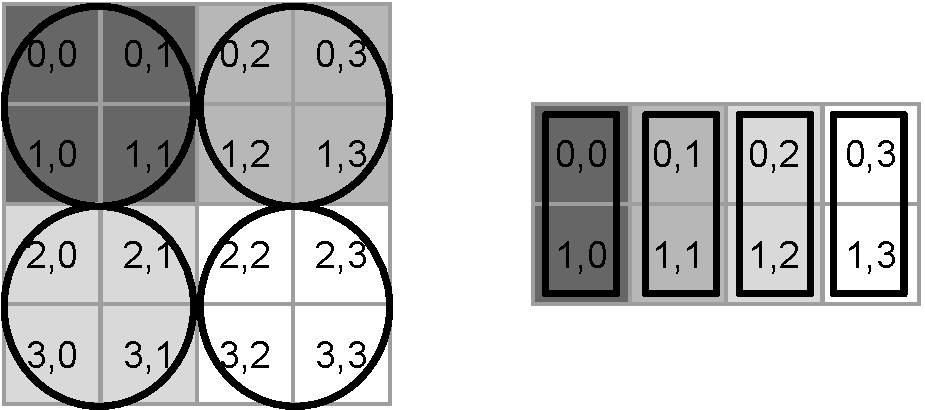
\includegraphics[width=85mm]{pictures/example}
\caption {A geometry mapping example, the left matrix is input and the right matrix is output. The mapping between the geometries are shown using gray shades.
    \label{fig:example}
}
\end{center}
\end{figure}


\begin{table}[h]
\begin{center}
    \caption{Element-wise mapping and geometry mapping of the example in Figure~\ref{fig:example}}
    \begin{scriptsize}
    \begin{tabular}{ | c | c | c | c |}
    \hline
    Input & Geometry & Output & Geometry \\ \hline \hline
    (0,0),...,(1,1) & Circle\_0 & (0,0),(1,0) & Rect\_0 \\ \hline
    (0,2),...,(1,3) & Circle\_1 & (0,1),(1,1) & Rect\_1 \\ \hline
    (2,0),...,(3,1) & Circle\_2 & (0,2),(1,2) & Rect\_2 \\ \hline
    (2,2),...,(3,3) & Circle\_3 & (0,3),(1,3) & Rect\_3 \\ \hline
    \end{tabular}
    \end{scriptsize}
    \label{tb:example}
\end{center}   
\end{table} 

\subsubsection{No Index}
Using the example in Table~\ref{tb:example}, with {\bf NoIndex} strategy, a query for an element needs to traverse all circles (input geometries).
If the element is in a circle, the query returns the all output elements expanded from the mapping rectangle.
The time complexity of a query is $O(N)$, where $N$ is the number of circles. 

\subsubsection{Direct Index}
To build the {\bf Direct} index, SystemX uses each input element as key and the associated geometry as the value, as shown in Figure~\ref{fig:direct}.
SystemX relies on the underlying runtime system for the optimization of storing repeated geometries as a single object,
then uses a pointer (hash value) of the geometry object, as shown in Figure~\ref{fig:direct-optimized}.
A query of an element takes two steps: the first step returns the hash value for that element and the second step returns the rectangle. 
The space complexity of {\bf Direct} index is $O(N*M)$, where $N$ is the number of circles and $M$ is the number of elements in each circle.
The time complexity of building index and query are $O(N*M)$ and $O(1)$, respectively.

\begin{figure}
\centering
\begin{minipage}{.3\linewidth}
  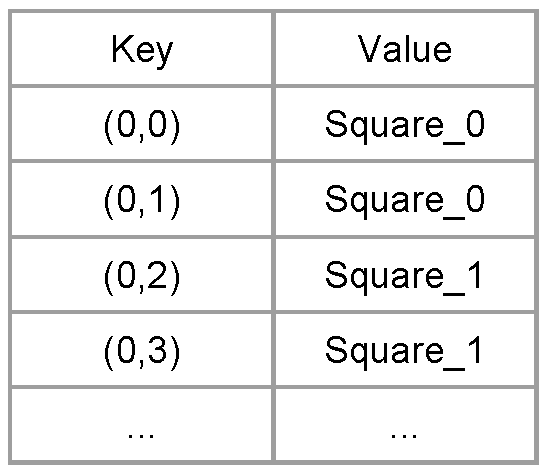
\includegraphics[width=\linewidth]{pictures/direct}
  \caption{Direct index}
  \label{fig:direct}
\end{minipage}
\hspace{.05\linewidth}
\begin{minipage}{.6\linewidth}
  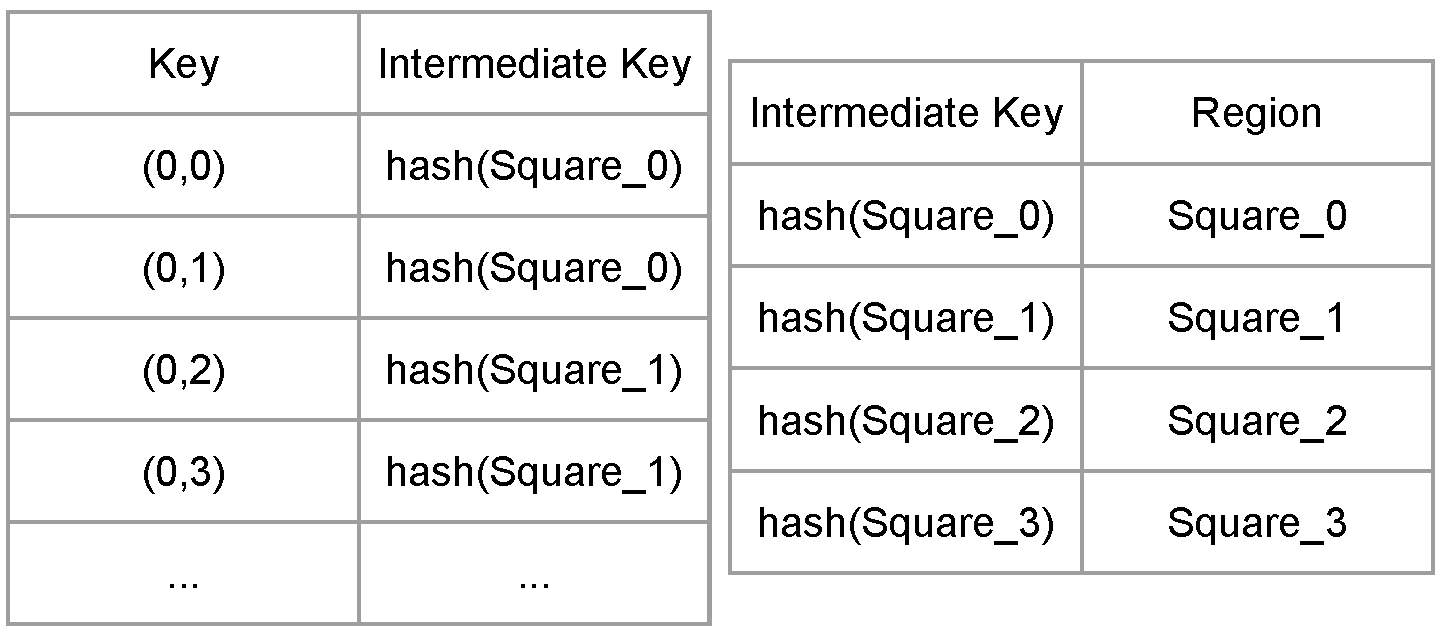
\includegraphics[width=\linewidth]{pictures/direct-optimized}
  \caption{Direct index with optimization}
  \label{fig:direct-optimized}
\end{minipage}
\end{figure}


\subsubsection{RTree Index}
R-tree~\cite{guttman1984} has been introduced to index multidimensional information.
To simplify the discussion, SystemX uses the example shown in Figure~\ref{fig:example} and build the index in a two dimensional space.
The average query time complexity is $O(logN)$, while the worst case is $O(N)$. 
The worst case happens when querying an element in a region where all leaf nodes overlap.
Variants of R-tree, such as R+-tree~\cite{sellis1987} and R*-tree~\cite{beckmann1990}, 
seek to improve the worst case query by minimizing the overlapped geometry at leaf nodes 
by paying the index building cost.

In our use cases, it is rare that a single element occurs in all geometries.  
R-tree is sufficient to validate the idea of using spatial indexing for geometry mapping.

SystemX uses an open source Archery~\cite{osheim13} to build the {\bf RTree} index.
In the Archery implementation, both the leaf nodes and the non-leaf nodes are abstracted as rectangles.
To differentiate from the rectangle geometries, an Archery rectangle is referred as a box.
To adapt the geometry to Archery, SystemX firstly computes the bounding box of each circle, then uses
a tuple of the bounding box and the circle as leaf node of the R-tree. 
The index is built upon the bounding boxes. 
The query of an input element (0,0) in the R-tree returns a tuple of the bounding box (center: (0.5,0.5), height:1, width:1) and circle\_0.
The query returns the output elements expanded from Rect\_0 only if the input element is within circle\_0.

The time complexity in worst case of insertion an R-tree is $O(N)$.
The worst case time complexity of query an R-tree is $O(N)$.
And the space complexity for {\bf RTree} index is $log(N)$.

\subsubsection{KMeans Index}
We design a two-layer tree index with its leaf nodes as a list of geometries and its non-leaf nodes as the bounding box (same idea as that of R-tree)
of all geometries in the list.
The geometries are distributed to each non-leaf node using the KMeans~\cite{macqueen67} algorithm.

This {\bf KMeans} strategy clusters $N$ geometries into $\sqrt{N}$ clusters, 
since $\sqrt{N}$ is the optimal cluster number for the worst case query when N geometries are uniformly distributed in a two dimensional space.
Clustering $N$ geometries into $k$ clusters results in $\frac{N}{k}$ elements in each cluster. 
Thus there are $k$ non-leaf nodes.
A worst case query needs to traverses all $k$ non-leaf nodes and all $\frac{N}{k}$ leaf node in the cluster.
$k+\frac{N}{k}$ has its minimum when $k=\sqrt{N}$. 

The time complexity of building the {\bf KMeans} index is $O(N^{1.5})$.
The worst case query time complexity is $O(\sqrt{N})$.
The space complexity of {\bf KMeans} is $O(\sqrt{N})$.

%\subsubsection{Index Strategy Asymptotical Comparison}
%Table~\ref{tb:index-comparison} summarizes the index building time complexity, 
%the query time complexity, and the index space complexity.
%
%\begin{table}[t]
%\begin{center}
%    \caption{Index Strategy Comparison}
%    \begin{scriptsize}
%    \begin{tabular}{ | c | c | c | c |}
%    \hline
%    Strategy & Building & Worst Query & Space \\ \hline \hline
%    NoIndex & 0 & $O(N)$ & 0 \\ \hline
%    Direct & $O(N^2)$ & $O(1)$ & $O(N^2)$ \\ \hline
%    RTree & $O(N)$ & $O(\sqrt{N})$ & $O(logN)$ \\ \hline
%    KMeans & $O(N^{1.5})$ & $O(N)$ & $O(\sqrt{N})$ \\ \hline
%    \end{tabular}
%    \end{scriptsize}
%    \label{tb:index-comparison}
%\end{center}   
%\end{table}
%
%{\bf Direct}'s query performance is the best from analysis, however the building time overhead and space overhead is quite high.
%{\bf RTree} and {\bf KMeans} have a more balanced building time, space and query performance.
%In reality, we see the performance of {\bf RTree} an {\bf KMeans} are significantly affected by parameters such as the
%number of boxes in each non-leaf node for {\bf RTree} and the number of iterations for {\bf KMeans}.
%A detailed performance study is present in \S\ref{sec:Perf-Index}.

%\begin{table}[t]
%\begin{center}
%    \caption{Index Strategy Profile on Single SIFTExtracror}
%    \begin{scriptsize}
%    \begin{tabular}{ | p{1.7cm} | p{0.9cm} | p{0.8cm} | p{0.9cm} | p{1cm} | p{1cm} |}
%    \hline
%    Strategy & NoIndex & Direct & RTree & KMeans1 & KMeans5 \\ \hline \hline
%    Average (ms) & 0.28 & 0.04 & 0.095 & 0.073 & 0.049 \\ \hline
%    Stdev & 0.08 & 0.011 & 0.022 & 0.011 & 0.014 \\ \hline
%    Space (MB) & 0.44 & 22.49 & 0.78 & 0.5 & 0.5 \\ \hline
%    \end{tabular}
%    \end{scriptsize}
%    \label{tb:single-SIFT-query}
%\end{center}   
%\end{table}

\section{Evaluation}
\label{sec:Perf}
In this section, we evaluate a number of aspects of SystemX's performance.
For geometry mapping indexing strategies, we measure the index building time, query performance, memory usage and storage consumption.
Then we present SystemX's lineage capturing performance with two real ML pipelines on varying cluster sizes.
We also measure the performance of the three use cases presented in \S\ref{sec:Back-cases}.

All experiments are run on Amazon EC2 using r3.8xlarge instances.
Each machine has 16 physical cores, 244 GB memory, and two 320GB SSD. 
SystemX is integrated with KeystoneML 0.3 which in turn runs over Spark 1.3.1 and 
HDFS from the CDH4 distribution of Hadoop. 

The two pipelines we are using are SIFTFisher and SourceExtractor. 
The datasets are VOC2007~\cite{pascal-voc-2007} and a subset of Sloan Digital Sky Survey~\cite{york00} (SDSS) Data Release 7, respectively.
Table~\ref{tb:datasets} summarizes the size and number of files of the datasets.

\begin{table}[t]
\begin{center}
    \caption{Data Size of SIFTFisher and SourceExtractor with the Meta-only and Meta+Data settings}
    \begin{scriptsize}
    \begin{tabular}{ | c | c | c | }
    \hline
    Dataset & Size & File Count \\ \hline \hline
    VOC& 828~MB &10,000  \\ \hline
    SDSS DR7 & 65~GB & 11,150 \\ \hline
    \end{tabular}
    \end{scriptsize}
    \label{tb:datasets}
\end{center}   
\end{table}

\subsection{Geometry Mapping Index}
\label{sec:Perf-Index}
With this experiment we seek to profile the query latency, lineage capturing time, memory usage and storage space 
of the indexing strategies for geometry mapping discussed in \S\ref{sec:GeometryIndex}.
In particular, KMeans-1 builds the index with one iteration while KMeans-5 builds the index with five iterations.
We use a workload derived from the SIFTExtractor transformer in the SIFTFisher pipeline. 
The mapping has 5,000 pairs of input and output matrix, with each pair producing 60,000 geometry tuples (300 million in total) that are uniformly distributed
in a 2D space. 
The experiment is executed on a 16 machine cluster.

Figure~\ref{fig:sift-query} presents the query performance with these indexing strategies.
For each strategy, we run queries with \{1, 100, 1K, 10K\} keys.
The Direct strategy crashes due to insufficient memory.
NoIndex strategy shows a high query latency which quickly grows over 10,000~ms with 100 keys.
The other three strategies show a similar scalability, while KMeans-1 runs 17.9\% and 25.1\% faster than RTree with 1K and 10K keys, respectively.
KMeans-5 runs  31.1\% and 35.2\% faster with 1K and 10K keys, respectively.
%This result is as expected as the Archery implementation hard codes the number of objects as 50 for each leaf node, which results in a deep tree.
%While the KMeans strategies are building two-level trees.

\begin{figure}[t]
\begin{center}
    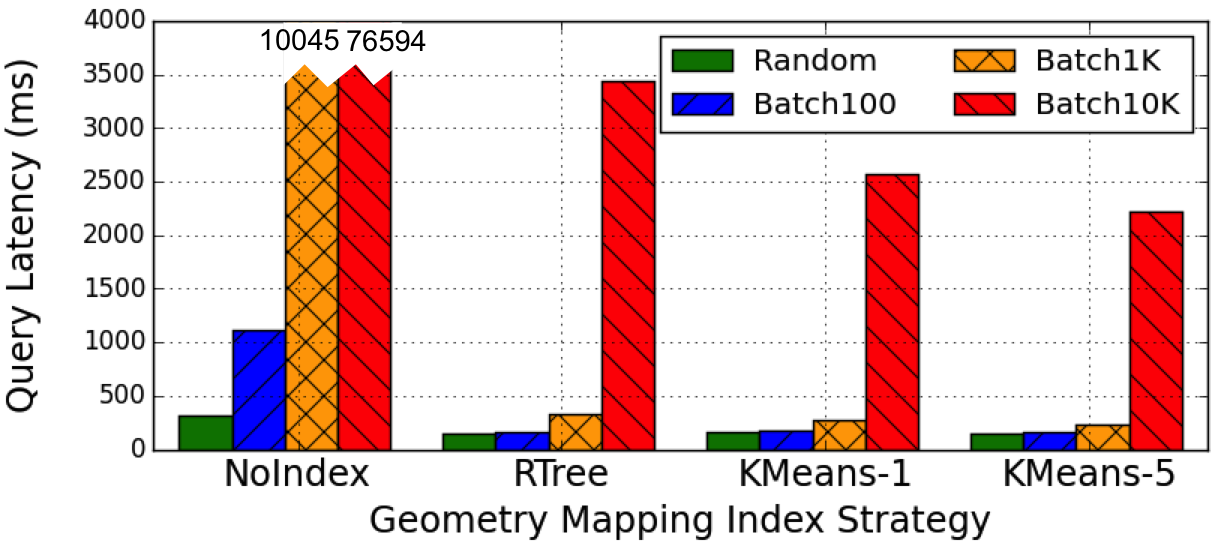
\includegraphics[width=85mm]{pictures/SIFTQuery-Time-tuned}
\caption {Query performance profile of the geometry mapping with four indexing strategies
    \label{fig:sift-query}
}
\end{center}
\end{figure}

Figure~\ref{fig:sift-time} presents the wall clock time of this workload with a detailed runtime decomposition. 
Capturing 300 million geometry tuples takes 89.8~seconds overhead in average. 
Building the index for these mappings takes 33.9, 69.9, and 349.0~seconds for RTree, KMeans-1, and KMeans-5, respectively.
Table~\ref{tb:sift-index-resource} presents the additional memory usage, storage space for mappings and
index separately.

\begin{figure}[t]
\begin{center}
    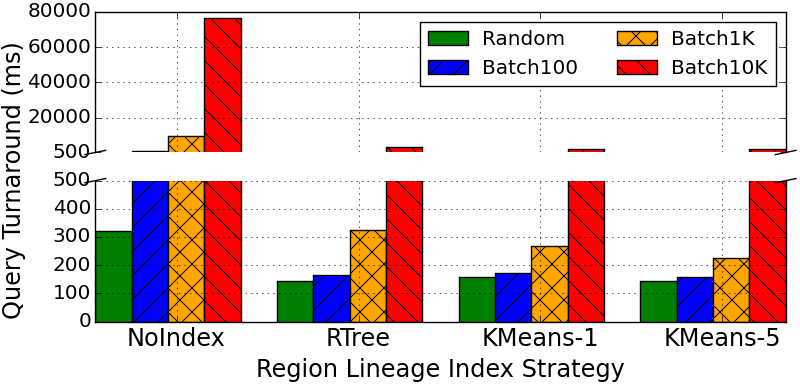
\includegraphics[width=85mm]{pictures/SIFTIndex-Time}
\caption {Runtime profile of the indexing strategies for geometry mapping with over 300 million pairs.
    \label{fig:sift-time}
}
\end{center}
\end{figure}


\begin{table}[t]
\begin{center}
    \caption{Summary of Additional Memory Usage (over 0.7~TB), Mapping Storage Space, and Index Storage Space for the Four Indexing Strategies}
    \begin{scriptsize}
    \begin{tabular}{ | c | c | c | c |}
    \hline
    Index & Additional  Mem & Mapping Space & Index Space \\ \hline \hline
    NoIndex & 71.4\% & 30.8~GB & 0 \\ \hline
    RTree & 85.7\% & 30.8~GB & 24.6~GB\\ \hline
    KMeans-1 & 85.7\% & 30.8~GB & 3.5~BG\\ \hline
    KMeans-5 & 114.3\% & 30.8~GB & 3.5~GB\\ \hline
    \end{tabular}
    \end{scriptsize}
    \label{tb:sift-index-resource}
\end{center}   
\end{table}


To summarize, NoIndex has the highest query latency and it is not practical for real use.
KMeans-5 has the best query performance and the longest index building time.
RTree has a balanced query performance and building time with the highest storage consumption.
Since storage is not the major bottleneck given the machine capability, SystemX uses the RTree strategy
as default, leaving the other strategies as users' options.


\subsection{Lineage Capturing Performance}
We evaluate lineage capturing wall clock time with the SIFTFisher and SourceExtractor pipelines. 
The goal is to evaluate if lineage capturing is scalable with larger cluster size in a strong scaling manner.
For each pipeline, we measure the wall clock time of lineage capturing with two settings.
With the first setting (meta-only), SystemX only captures the metadata mapping, since this is the minimal lineage information 
to preserve the pipeline lineage integrity.
With the second setting (meta+data), SystemX captures both the metadata mapping and the output dataset of each transformer.
With the lineage information captured in this way, queries on the output dataset does not require any rerunning of data transformations.
This is considered as the maximal lineage information of a pipeline. 
Table~\ref{tb:apps-stats} presents the dataset size collected with both settings for both pipelines.

\begin{table}[t]
\begin{center}
    \caption{Data Size of SIFTFisher and SourceExtractor with the Meta-only and Meta+Data settings}
    \begin{scriptsize}
    \begin{tabular}{ | c | c | c| }
    \hline
    Pipeline & SIFTFisher & SourceExtractor \\ \hline \hline
    Meta-only & 109.9~GB & 204.4~MB \\ \hline
    Meta+Data & 615.7~GB & 506.9~GB \\ \hline
    \end{tabular}
    \end{scriptsize}
    \label{tb:apps-stats}
\end{center}   
\end{table}

Figure~\ref{fig:VOC-overhead} shows the isolated wall clock time of lineage capturing of the SIFTFisher pipeline. 
From small scale to large scale, the meta-only setting scales up to 16 machines then flattens. 
On the other hand, the meta+data setting shows a better scalability since this is a relatively more
data-intensive procedure compared to the meta-only setting. 
By examining the pipeline measurements, we confirm that the scalability of the meta-only setting is bounded
by the pipeline performance.
From 4 to 8 machines, the meta-only setting shows a super linear speedup, this is because the pipeline is memory-bounded on 4 machines
and using 8 machines removes this bottleneck.

On 16 machines, the SIFTExtractor counts for 89.4\% of the 226~seconds wall clock time cost in the meta-only case.
This is because it is instrumented as the geometry mapping type.
It implies that all other SystemX's mapping types have low cost to be captured.
The rest of the transformers contribute a total of 10.6\% in this pipeline. 

\begin{figure}[t]
\begin{center}
    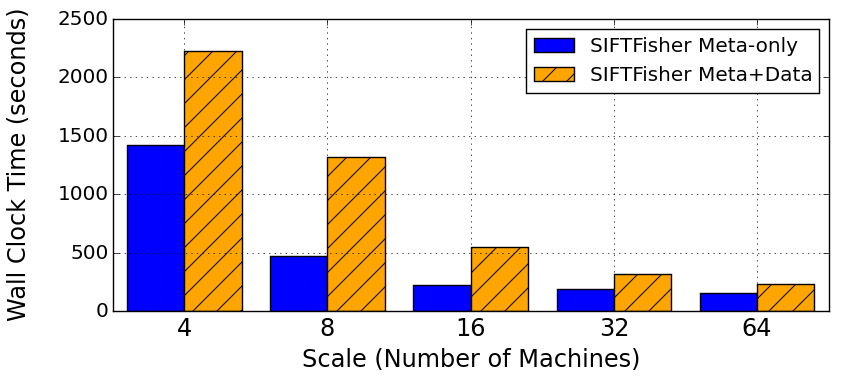
\includegraphics[width=85mm]{pictures/Overhead-Time-VOC}
\caption {Isolated Lineage Capturing Wall Clock Time of the SIFTFisher Pipeline
    \label{fig:VOC-overhead}
}
\end{center}
\end{figure}

Figure~\ref{fig:SE-overhead} shows the isolated wall clock time cost of lineage capturing of the SourceExtractor pipeline.
By profiling the SourceExtractor's lineage-free performance, we observe that this pipeline's runtime only improves by 5.5\% from 8 machines
to 16 machines. Then the performance starts to slow down with larger scale.
Given the poor scalability of the SourceExtractor pipeline, the meta-only setting performance is bounded by the pipeline scalability.
While the Meta+Data setting scales better due to its nature of data intensiveness.
An analysis on the 8 machine performance shows that the Extractor contributes 87.6\% of the cost when SystemX only captures metadata mapping.
This is because the Extractor transformer records its lineage as geometry mapping.
\begin{figure}[t]
\begin{center}
    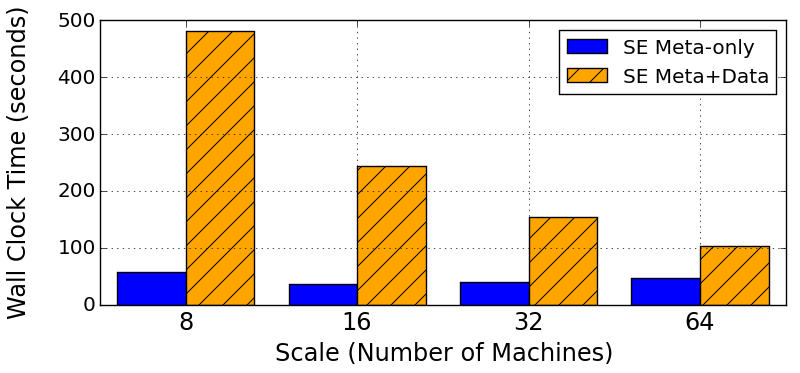
\includegraphics[width=85mm]{pictures/Overhead-Time-SE}
\caption {Isolated Lineage Capturing Wall Clock Time of the SourceExtractor Pipeline
    \label{fig:SE-overhead}
}
\end{center}
\end{figure}

One pattern we can conclude from the scalability measurements is that SystemX's lineage capturing wall clock 
time scales better than or similar to the ML pipelines.
This is due to the fact that SystemX captures and stores the lineage in a distributed manner. 
The metadata mapping capturing is more likely to be impacted by the ML pipeline compared to the case where both metadata
mapping and datasets are captured, since it is a relatively less data-intensive procedure.
For both pipelines, geometry lineage dominates the wall clock time overhead when only capturing the metadata mapping.


\subsection{Query Latency and Scalability}
In some cases, a user is only interested in one element of a single transformer.
The query is then in the form of random query with a single key.
While with a sequence of transformers, an individual element forward query 
can return a large number of coordinates, e.g., 1~million, from the first transformer. 
Then the subsequent query has to use these 1~million coordinates as keys.
This large key number on a single data structure can impact the query performance substantially.  
This performance measurement seeks to profile the query scalability boundary of SystemX on a single data structure in terms of key number. 

We run queries with varying key numbers and present the performance in Figure~\ref{fig:typequery}. 
For each lineage type, we use a collection of 5,000 pairs of 
input and output data structures (vector, matrix, image) and distribute them over 16 machines.
Table~\ref{tb:typequery-stats} shows the metadata settings of the input and output data structure in each query

\begin{figure}[t]
\begin{center}
    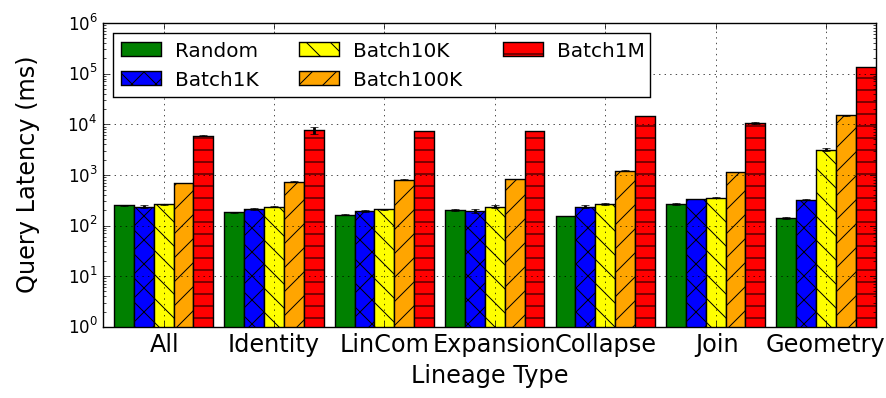
\includegraphics[width=85mm]{pictures/TypeQuery-Time}
\caption {Query latency for the seven lineage types (in log scale).
    \label{fig:typequery}
}
\end{center}
\end{figure}

\begin{table}[t]
\begin{center}
    \caption{Data Structure Settings}
    \begin{scriptsize}
    \begin{tabular}{ | c | c | c |}
    \hline
    Type & Input Structure & Output Structure \\ \hline \hline
    All & Vector(40960) & Vector(40960) \\ \hline
    Identity & Matrix(80, 512) & Matrix(80, 512) \\ \hline
    LinCom & Vector(40960) & Vector(20) \\ \hline
    Flatten & Matrix(80, 512) & Vector(40960) \\ \hline
    Collapse & Image(375, 500, 3) & Matrix(375, 500) \\ \hline
    Join & Matrix(500, 300) & Matrix(300, 500) \\ \hline
    Geometry& \shortstack[l]{Matrix(300, 500), \\60K geometries} &  \shortstack[l]{Matrix(128, 60000), \\60K geometries} \\ \hline
    \end{tabular}
    \end{scriptsize}
    \label{tb:typequery-stats}
\end{center}   
\end{table}

Given the fact that all mapping, identity mapping, lincom mapping, flatten mapping, collapse mapping, and join mapping
only involve trivial computation, queries with 1 to 10K keys show latency under 200~ms. 
These queries show performance degradation with 100K keys (around 1~second). 
From 100K keys, the query latency increases proportionally with the key number as shown with the 1M key performance.
Geometry Mapping shows a consistent latency under 200~ms from 1 to 1K keys. 
Beyond that, a query with 10K keys takes $2.41\pm0.6$~seconds and a query with 1M keys take $132.9\pm0.4$~seconds

This query scalability profile shows low latency ($\sim$200~ms) for an element investigation on one data structure tuple. 
With the end-to-end pipeline lineage, the query can be slow due to the quickly increasing key number.
One such case on an hand-written digit classification pipeline with 16 chained transformers 
takes $1\pm0.1$~seconds for backward query and $1.0\pm0.05$ for forward query.
While in the case of SIFTFisher pipeline,  it can take an estimated $O(10^3)$~seconds to finish as the backward query on the SIFTExtractor
transformer can have a key count of 7.7M.
The actual mapping is from a matrix with 128 rows and 60K columns to an image with 333 rows, 500 columns and 3 channels. 
For the moment, we leave the optimization of large scale query on single data structure as future work.

\subsection{Use Case}
In the {\bf code validation} case, users instrument the SIFTFisher pipeline by only capturing the metadata mapping of the SIFTExtractor transformer.
Upon validation, users can query extracted feature, and locate the positions of the corresponding pixels in the input image. 
With some external visualization tool, users can visualize these pixels in the original image. 
Such an instrumentation introduces a wall clock time overhead of 15.8\% on a 16 machine cluster.
Query a single feature takes $0.14\pm0.0062$~seconds while a batch query of 1,000 features takes $0.33\pm0.001$~seconds.

In the {\bf results inspection} use case, users of the SourceExtractor pipeline captures the metadata mapping in all transformers along with the output 
datasets of the Extractor transformer. By joining the metadata mapping with the output dataset, which contains the luminosity information, users can first filter out the
objects with a threshold brightness. Then the user queries the metadata mapping to find the positions of corresponding pixels in the input images.
This instrumentation introduces a wall clock time overhead of 40.8\% on a 8 machine cluster. 
Filtering {\it luminous flux >300,000~lumen} over 1 million objects returns 10,283 objects
with the corresponding pixel positions in $1.84\pm0.14$~seconds. 
A forward query that traces the error propagation given a bad pixel takes $3.3\pm0.03$~seconds to return.

In the {\bf data cleaning} use case, the user of the SIFTFisher pipeline wants to remove the training images that have both the dogs and cats.
So he instruments the pipeline to capture all metadata mappings and the output datasets for NormalizeRows transformer. 
Upon removal, he first joins the output dataset of NormalizeRows (a RDD of vectors) with the labels.
Then he filters out the corresponding vectors with both cats and dogs in it ( eight vectors corresponding to eight images in this case). 
From here, he can try retrain the model with the cleaned dataset. 
This particular instrumentation introduces a wall clock time overhead of 46.8\%, and the removal takes $25.7\pm0.27$ seconds.
Compared to the case of rerunning the data preparation phase of the pipeline, using lineage information speeds up the turnaround
time by 16.4x (from $421.3\pm3.8$~seconds to $25.7\pm0.3$~seconds). 


\section{Related Work}
\label{sec:Related}
{\bf Coarse-grained Lineage:} Researchers have extensively studied data lineage (in some cases referred as data provenance) in different contexts.
Scientific workflow systems such as  Chimera~\cite{foster02}, Taverna~\cite{oinn02}, and ESSW~\cite{frew01}, 
collect coarse-grained lineage of file metadata and computation. 
Similar work has been well summarized by surveys~\cite{simmhan05, freire08, bose05}.
Recent work by Altintas~\cite{altintas10} investigates how to integrate the lineage of workflow executions
in a collaborative environment. Coarse-grained lineage is useful in these systems to trace the data and code dependencies.
However, the coarse-grained lineage lacks the details at cell level for ML pipelines diagnosis.

{\bf Fine-grained Lineage:} Fine-grained lineage has been investigated in the context of data visualization~\cite{stonebraker93, woodruff97},  
data warehouse~\cite{cui00, cui03}, RDBMS~\cite{widom04}, and user-curated database~\cite{buneman06}.
Recent works of RAMP~\cite{ikeda11, park11} and Newt~\cite{logothetis13} capture fine-grained lineage for the MapReduce
systems. SubZero~\cite{wu13} proposes a lineage system for the array-based SciDB~\cite{brown10}.
All these systems design lineage capturing interface on the well-defined low level operators.
For example, the data warehouse has the aggregate, select, project, join operators. 
RDMBS has its SQL operators. MapReduce systems formulates the computation as mappers and reducers.
The curated database defines four operators of insert, delete, copy and paste.
Though lineage capturing interface designed in these systems is general to support all applications running on top them,
they are not suitable for the ML pipeline diagnostics.
This is because ML frameworks do not have such a set of well-defined low level operators since an ML pipeline is a sequence of user-defined 
data transformations.

One of SubZero's contributions is the region lineage that collects fine-grained lineage for UDFs besides the built-in operators in SciDB. 
However, region lineage is not sufficient for ML pipelines because it only captures many to one relationships between input and output cells, 
while ML pipelines require many to many relationships as well.

{\bf Other Fine-grained Lineage Capturing Techniques:} Researchers also have tried to collect fine-grained lineage with other approaches.
Weak inversion and verification methods~\cite{woodruff97} are proposed to support approximate lineage collection.
Dynamic program analysis is employed to capture fine-grained lineage inside non-relational operators~\cite{zhang07} with 
a 7.5$\sim$39.8x slowdown compared to the original program. 
%DeepDive~\cite{shin15} explores approximate inference for the incremental maintenance problem in the context of knowledge base system.
These approaches do not fit the ML pipeline lineage scenario since they either lose the lineage accuracy or introduce
excessive performance penalty.
The Arnold system~\cite{devecsery14} captures fine-grained lineage at operating system process level by recoding
all non-deterministic data such as the order, return values, modified memory addresses, and many others. 
This approach can collect fine-grain lineage for any process in the operating system, however
it loses track of the upper level data structures (e.g., vector, matrix, images), which are fundamental to ML pipelines.
One step beyond fine-grained lineage, researches~\cite{meliou10, meliou11} explore the causality and responsibility
of inputs to the results. Though the causality and responsibility is relatively easier for data transformations in ML pipelines,
such techniques can be applied in the training process analysis to infer the contribution of individual training sample to the 
model and predictions.


\section{Conclusion and Future Work}
\label{sec:Conclusion}
SystemX enables interactive ML pipeline diagnostics by leveraging the fine-grained data lineage.
SystemX exposes an elegant and powerful interface for users to specify and instrument lineage capuring.
This interface has a coverage of 87\% of the transformers in the current KeystoneML code base. 
Combining the metadata of data structures, the high-order function approach and spatial indexing
strategy, SystemX is able to answer typical queries within a few seconds. 
Practically, SystemX introduces a wall clock time overhead of 16\%-54\% depending on the pipeline 
and use case.

As future work, we are investigating the diagnosability inside the training process of the estimator. 
We seek to provide users with the fine-grained lineage for an estimator to answer queries such as
finding supporting training samples for a prediction and the impact of certain feature removal or training data item removal. 
We are also working on the optimization of large scale query on a single data structure.

%ACKNOWLEDGMENTS are optional
\section{Acknowledgments}
This research is supported in part by NSF CISE Expeditions Award CCF-1139158, LBNL Award 7076018, and DARPA XData Award FA8750-12-2-0331, and gifts from Amazon Web Services, Google, SAP,  The Thomas and Stacey Siebel Foundation, Adatao, Adobe, Apple, Inc., Blue Goji, Bosch, C3Energy, Cisco, Cray, Cloudera, EMC, Ericsson, Facebook, Guavus, Huawei, Intel, Microsoft, NetApp, Pivotal, Samsung, Splunk, Virdata, VMware, and Yahoo!. 

%
% The following two commands are all you need in the
% initial runs of your .tex file to
% produce the bibliography for the citations in your paper.
\bibliographystyle{abbrv}
\balance
\bibliography{Lineage} % sigproc.bib is the name of the Bibliography in this case
% You must have a proper ".bib" file
%  and remember to run:
% latex bibtex latex latex
% to resolve all references
%
% ACM needs 'a single self-contained file'!
%
%APPENDICES are optional
%\balancecolumns



\balancecolumns

% That's all folks!
\end{document}
